\documentclass[a4paper]{article}
\usepackage{ctex}
\usepackage{tikz}\usetikzlibrary{arrows,calc,intersections,through,backgrounds,math,angles,shapes}
\usepackage{hyperref}
\usepackage{amsmath,amssymb,mathrsfs}
\usepackage[includemp=true,marginparsep=.5cm,marginparwidth=3cm,left=2.5cm,right=2cm]{geometry}%带旁注
\def\sky{\par\vspace*{1ex}}
\newcommand\tbs[1][]{\tt\char`\\#1}
\newcommand\Dd{\displaystyle}
\newcommand\bpics[1]{\par\vspace{1ex}\noindent\begin{minipage}{\textwidth}\begin{minipage}{#1\textwidth}}
\newcommand\mpics[1]{\end{minipage}\begin{minipage}{#1\textwidth}\linespread{1}}
\newcommand\epics{\end{minipage}\end{minipage}\par\vspace{2ex}}
\begin{document}
\tableofcontents
\section{字符输入}
    \TeX 系统中有些字符用于控制系列,不可以直接输入。\par
    \begin{tabular}{|c|c|c|c|c|c|c|c|c|c|}\hline
      输入 & \tbs{\char35} & \tbs{\char36} & \tbs{\char37} & \tbs{\char38} & \tbs{\char123} & \tbs{\char125} & \tbs{\char95} & \tbs{\char94\{\}} & \tbs{\char126\{\}} \\ \hline
      显示 & \# & \$ & \% & \& & \{ & \} & \_ & \^{} & \~{} \\ \hline
      输入 & \multicolumn{2}{|c|}{\tbs{textless}} & \multicolumn{2}{|c|}{\tbs{textgreater}} & \multicolumn{2}{|c|}{\tbs{textbar}} & \multicolumn{3}{|c|}{\tbs{textbackslash}}\\ \hline
      输出 & \multicolumn{2}{|c|}{\char60} & \multicolumn{2}{|c|}{\char62} & \multicolumn{2}{|c|}{\char124} & \multicolumn{3}{|c|}{\char92} \\ \hline
    \end{tabular}
\section{字体}
  \subsection{字型编码:encoding}
    字型编码即各个个别的字在一个字型里头的排列顺序以及安排方式。原始的 \TeX 字型编码我们就称为 OT1(Old TEX text encoding), 这是预设的, 如果都不指定字型编码, 那所使用的就是 OT1 编码。
  \subsection{字族:family}
    \begin{tabular}{|l|l|l|}
            \hline
            命令式 & 环境式 & 描述\\
            \hline
            \tbs{textrm}\{text\} & \{\tbs{rmfamily} text\} & roman字族 \\
            \hline
            \tbs{textsf}\{\textsf{text}\} & \{\tbs{sffamily} \textsf{text}\} & sans-serif字族 \\
            \hline
            \tbs{texttt}\{\texttt{text}\} & \{\tbs{ttfamily} \texttt{text}\} & monospace字族 \\
            \hline
          \end{tabular}

    \subsubsection{serif}
       罗马字体,又称衬线字体,字符笔画的起始处有装饰,利于阅读,为印刷专用字体。

      Serif 字体著名的有:Times New Roman、DejaVu Serif、宋体、明体等。
    \subsubsection{sans-serif}
       无衬线字体,又称等线字体,字符笔画的起始处无装饰,专用于荧幕、简报、艺术字体、展示等,较美观,但不适于长时间阅读。

      Sans-Serif 字体著名的有:DejaVu Sans、Helvetica、Verda-na、圆体、黑体等。
    \subsubsection{monospace}
      打字机字体,又称等宽字体,每个英文字母皆设计为同一宽度,以便于排版;现代为节省不必要空间的浪费,依字母形状分配其宽度。现多用于终端机显示、程序码表示等。

      Monospace 字体著名的有:Andale Mono、DejaVu SansMono 、Courier、AR PL New Sung Mono。
  \subsection{字型系列:series}
    \begin{tabular}{|l|l|l|}
      \hline
      命令式 & 环境式 & 描述\\
      \hline
      \tbs{textmd}\{text\} & \{\tbs{mdseries} text\} & 正常字体粗细 \\
      \hline
      \tbs{textbf}\{\textbf{text}\} & \bfseries\{\tbs{bfseries} \textbf{text}\} & bold 粗体 \\
      \hline
    \end{tabular}

    正常用的是 medium,m。粗体是 bold,b。然后还有 Bold extended,bx。还有Semi-bold,sb。。和 Condensed,c
  \subsection{字形:shap}
    字形有正常的 normal,n。还有意大利斜体 Italic,it。斜体 Slanted,sl。和Small Caps,sc。

    \begin{tabular}{|l|l|l|}
      \hline
      命令式 & 环境式 & 描述\\
      \hline
      \tbs{textup}\{text\} & \{\tbs{upshape} text\} & 正常字形 \\
      \hline
      \tbs{textit}\{\textit{text}\} & \{\tbs{itshape} \textit{text}\} & 意大利斜体 \\
      \hline
      \tbs{textsl}\{\textsl{text}\} & \{\tbs{slshape} \textsl{text}\} & 斜体 \\
      \hline
      \tbs{textsc}\{\textsc{text}\} & \{\tbs{scshape} \textsc{text}\} & small caps \\
      \hline
    \end{tabular}
  \subsection{字号:size}
    {\tiny \tbs{tiny}}
    {\scriptsize\tbs{scriptsize}}
    {\footnotesize\tbs{footnotesize}}
    {\small\tbs{small}}
    {\normalsize\tbs{normalsize}}
    {\large\tbs{large}}
    {\Large\tbs{Large}}
    {\LARGE\tbs{LARGE}}
    {\huge\tbs{huge}}
    {\Huge\tbs{Huge}}
\section{长度}
\subsection{单位长度}
    \begin{tabular}{|ll|ll|}
      \hline
      单位 & 说明 & 单位 & 说明\\
      \hline
      pt & point() & bp & big point(1in=72bp)\\
      \hline
      pc & pica(1pc=12pt) & in & inch(1in=72.27pt)\\
      \hline
      cm & centimeter(1in=2.54cm) & mm & millimeter(1mm=2.84pt) \\
      \hline
      em & 当前字体中 M 的宽度 & ex & 当前字体中 x 的高度\\
      \hline
      mu & math unit, 1/18 em & sp & scaled poind(65536sp=1pt)\\
      \hline
    \end{tabular}
\subsection{长度命令}
    \tbs{newlength}\tbs{lengthname}:新建一个长度名

    \tbs{setlength}\tbs{lengthname}\{length\}:给长度量赋值

    \tbs{addtolength}\tbs{lengthname}\{length\}:在原有的长度上加上一个量

    长度命令定义后,可以使用\tbs{the}\tbs{lengthname}显示。
\section{段落}
  \subsection{换行与分段}
    \tbs{par} 命令表分段,一个空行当作 \tbs{par} 处理。一个换行符当作空格处理,多个空格当一个空格处理。另外在数学模式中空格全忽略。

    换行而不分段,用命令 \tbs\tbs。此命令后面可以跟上[10pt], 加上额外的间距,参数可为负。

    \tbs 后接一个空格,表示一个空格,在数学模式中也有效。

    由于换行被处理成一个空格,如果想去掉它,只需在行末加上 \%
  \subsection{段落对齐与间距}
    \LaTeX 中的段落缺省两端对齐 (fully justified) ,下面的三个环境可以让段落分别居左、居右或居中对齐,flushleft, flushright, center。另有三个命令 (\tbs{raggedleft}, \tbs{raggedright}, \tbs{centering}) 可以完成同样功能,这些命令还可以控制表格图片 (也许是一切盒子?) 的位置。

    段落首行缩进的距离可以用 \tbs{parindent} 变量来控制。

    段落之间的距离可以用 \tbs{parskip} 变量来控制。比如\\
    \verb|\setlength{\parskip}{1.6ex plus 0.2ex minus 0.2ex}|

    行间距是段落中相邻两行基线之间的距离,\LaTeX 缺省使用单倍行距。我们可以用 \tbs{linespread} 命令来控制行距。

    \tbs{linespread}\{1.3\} 表示一倍半行距 \quad \tbs{linespread}\{1.6\} 表示双倍行距。另外行间距是一个 glue,我们知道 glue有基本的 space 和伸缩量。行距的基本 space 由命令 baselineskip 控制,伸缩量有 baselinestretch 命令。分别用 \tbs{setlength} 和 \tbs{renewcommand} 来修改。如果要在文档中改变行间距必须采用如下的形式:\\
    \verb|{\linespread{伸缩量}\selectfont sometext \par}|
  \subsection{特殊段落}
    \LaTeX 中有三种摘录环境:quote, quotation, verse。quote 两端都缩进,quotation 在 quote 的基础上增加了首行缩进,verse 比 quote 多了第二行起的缩进。
\section{盒子}
  \subsection{盒子简述}
  在 \LaTeX 中每一个排版对象都是一个盒子。排版就是要把小盒子用空白间距粘在一起放到大盒子里,然后再依次嵌套到更大的盒子里。怎样优化这些大大小小的盒子是一门很深的学问。

  最小的盒子就是一个字符,这些字符然后组成更大的盒子---单词,然后单词组成更大的盒子---行等等。行是一个盒子,段落也是一个盒子,图片是一个盒子,表格也是一个盒子。而这些盒子按照 Knuth 的描述都是用 glue 胶水粘合起来的。下面就是一个盒子的详细参数:

  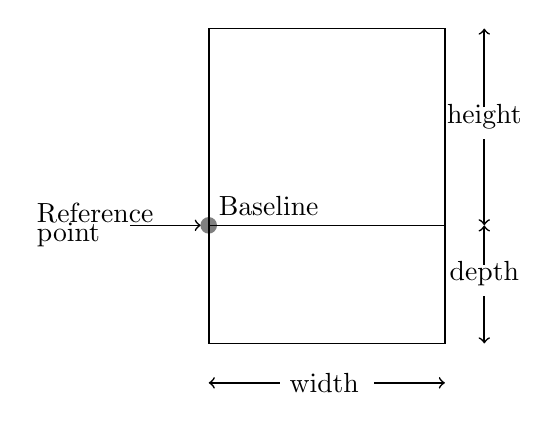
\begin{tikzpicture}[semithick]
    \draw[->](-1,0)--(-.1,0);
    \fill (0,0)node[left=1cm]{\parbox{3em}{Reference\\[-5pt]point}} [gray]circle (3pt);
    \draw(0,-1.5) rectangle (3,2.5);
    \draw(0,0)node[above right]{Baseline}--(3,0);
    \draw[<-](0,-2)--(.9,-2) node[right]{width};
    \draw[->](2.1,-2)--(3,-2);
    \draw[<-](3.5,0)--(3.5,1.1)node[above]{height};
    \draw[->](3.5,1.5)--(3.5,2.5);
    \draw[<-](3.5,-1.5)--(3.5,-.9)node[above]{depth};
    \draw[->](3.5,-.5)--(3.5,0);
  \end{tikzpicture}

  介绍两个 \TeX 命令。\tbs{hbox}让所有的盒子水平对齐,而 \tbs{vbox}把一些 hbox 竖直对齐。

  \subsection{简单盒子}
    最简单的盒子命令是 \tbs{mbox} 和 \tbs{fbox}。前者把一组对象组合起来,后者在此基础上加了个边框。

    黑色盒子可以用于画线条:\tbs{rule}[depth]\{width\}\{height\}
  \subsection{中等盒子}
    稍复杂的 \tbs{makebox} 和 \tbs{framebox} 命令提供了宽度和对齐方式控制的选项。其对齐方式有居中 (缺省) 、 居左、居右和分散对齐,分别用 c, l, r, s 来表示。

    语法:[宽度][对齐方式]\{内容\}

    raisebox 命令一般的用法就是:\tbs{raisebox}\{高度\}\{内容\}

    表示把某个内容放进一个盒子里然后抬高多少高度,高度值可以是负值则是降低。

    带颜色的盒子;\tbs{colorbox}\{yellow\}\{\colorbox{pink}{test}\}  \quad
    \tbs{fcolorbox}\{red\}\{pink\}\{\fcolorbox{red}{pink}{text}\}
  \subsection{高级盒子}
    盒子中的文本不能换行,大一些的对象比如整个段落可以用 \tbs{parbox} 命令或 minipage 环境,两者语法类似,有宽度、高度、外部对齐、内部对齐等选项。这里的外部对齐是指该盒子与周围对象的纵向关系,有三种方式:居顶、居中和居底对齐,分别用 t, c, b 来表示。内部对齐是指该盒子内部内容的纵向排列方式,也是同样三种。

    语法:[外部对齐][高度][内部对齐]{宽度}{内容}


\section{学习帮助}
    学习\LaTeX 开始时可以看入门的书籍,然后就需要看宏包的说明文档了。比如我要查看 xeCJK 文档,就在终端中输入:texdoc xeCJK
\section{数学公式}
  \subsection{数学模式}
    数学命令必须在数学模式中才能使用。数学模式有正文公式,如$(a+b)^2=a^2+2ab+b^2$,和行间公式,如
    \[\sum_{k=1}^nk=\frac{n(n+1)}{2}\]
    实现方式如下:\\
    \begin{tabular}{ccccc}
      \hline
       & \TeX 命令 & \LaTeX 命令 & \LaTeX 环境 & amsmath 环境 \\
      \hline
       行间公式 & \verb+$...$+ & \verb+\(...\)+ & math & \\
       行间公式 & \verb+$$...$$+ &\verb+\[...\]+ & displaymath & equation*\\
       编号行间公式 & & & equation &equation\\
      \hline
    \end{tabular}

    有时希望在正文中实现行间公式的效果,可用 \verb+\displaystyle+实现。另有同类命令 \verb+\textstyle\scriptstyle\scriptscriptstyle+ 分别实现文中、下标、下下标的效果。
  \subsection{上下标}
    下标用\verb+_+表示,如\verb+a_1+输出$a_1$,当下标多于一个字符时用大括号,如 \verb+a_{ij}+输出$a_{ij}$, 而 \verb+a_ij+ 输出 $a_ij$. 上标用\verb+^+表示,可与下标一起使用,如\verb+a_1^2或a^2_1+ 输出$a_1^2$.

    在行间公式中上下标遇到 \verb+\sum+ 之类的命令会调整为 $\displaystyle \sum_{k=1}^n$ (\verb+\sum_{k=1}^n+).
  \subsection{根号}
    $\sqrt2 \quad \sqrt{a} \quad \sqrt[3]{a+b}$ \quad \verb|\sqrt2 \sqrt{a} \sqrt[3]{a+b}|
  \subsection{分数}
    $\frac12 \quad \frac{a}{b+c} \quad \dfrac ab$ \quad \verb|\frac12 \frac{a}{b+c} \dfrac ab|
    \verb|\dfrac| 可以在文中公式中显示行间公式的效果。

    $\binom{m}{k}$ \quad \verb|\binom{m}{k}|

  \subsection{求和等}
    \begin{tabular}{ll}
      $\sum_{k=1}^n k$ & $\sum\limits_{k=1}^n k$ \\
      \verb|\sum_{k=1}^n k| & \verb|\sum\limits_{k=1}^n k|\\
      $\Dd\sum_{k=1}^n k$ & $\sum\nolimits_{k=1}^n k$\\
      \verb|\sum_{k=1}^n k| & \verb|\sum\nolimits_{k=1}^n k|\\
    \end{tabular}

    类似的还有 \verb|\prod \lim \int|
  \subsection{向量}
    $\vec{a}$  \quad \verb|\vec{a}| \quad $\overrightarrow{AB}$ \verb|\overrightarrow{AB}|

  \subsection{希腊字母}
    \noindent\begin{tabular}{llllllllll}
      \hline
      $\alpha$ & \tbs{alpha} & $\beta$ & \tbs{beta} & $\gamma$ & \tbs{gamma} & $\delta$ & \tbs{delta} & $\epsilon$ & \tbs{epsilon}\\
      $\varepsilon$ & \tbs{varepsilon} & $\zeta$ & \tbs{zeta} & $\eta$ & \tbs{eta} & $\theta$ & \tbs{theta} & $\vartheta$ & \tbs{vartheta}\\
      $\iota$ & \tbs{iota} & $\kappa$ & \tbs{kappa} & $\lambda$ & \tbs{lambda} & $\mu$ & \tbs{mu} & $\nu$ & \tbs{nu}\\
      $\xi$ & \tbs{xi} & $o$ & o & $\pi$ & \tbs{pi} & $\varpi$ & \tbs{varpi} & $\rho$ & \tbs{rho} \\
      $\varrho$ & \tbs{varrho} & $\sigma$ & \tbs{sigma} & $\varsigma$ & \tbs{varsigma} & $\tau$ & \tbs{tau} & $\upsilon$ & \tbs{upsilon}\\
      $\phi$ & \tbs{phi} & $\varphi$ & \tbs{varphi} & $\chi$ & \tbs{chi} & $\psi$ & \tbs{psi} & $\omega$ & \tbs{omega}\\
      \hline
      $\Gamma$ & \tbs{Gamma} & $\Delta$ & \tbs{Delta} & $\Theta$ & \tbs{Theta} & $\Lambda$ & \tbs{Lambda} & $\Xi$ & \tbs{Xi}\\
      $\Pi$ & \tbs{Pi} & $\Sigma$ & \tbs{Sigma} & $\Upsilon$ & \tbs{Upsilon} & $\Phi$ & \tbs{Phi} & $\Psi$ & \tbs{Psi}\\
      $\Omega$ & \tbs{Omega} & \$ & \tbs\$ \\
      \hline
    \end{tabular}
  \subsection{常用符号}
  \noindent
    \begin{tabular}{llllllllll}
      \hline
      $\pm$&\tbs{pm}&$\mp$&\tbs{mp}&$\times$&\tbs{times}&$\div$&\tbs{div}\\
      $\ast$&\tbs{ast}&$\le$&\tbs{le}&$\ge$&\tbs{ge}&$\equiv$&\tbs{equiv}\\
      $\cap$&\tbs{cap}&$\cup$&\tbs{cup}&$\sim$&\tbs{sim}&$\approx$&\tbs{approx}\\
      $\cong$&\tbs{cong}&$\neq$&\tbs{neq}&$\perp$&\tbs{perp}&$\in$&\tbs{in}\\
      $\subset$&\tbs{subset}&$\supset$&\tbs{supset}&$\subseteq$&\tbs{subseteq}&$\supseteq$&\tbs{supseteq}\\
      $\angle$&\tbs{angle}&$\infty$&\tbs{infty}&$\partial$&\tbs{partial}&$\triangle$&\tbs{triangle}\\
      $\prime$&\tbs{prime}&$\forall$&\tbs{forall}&$\exists$&\tbs{exists}&$\neg$&\tbs{neg}\\
      $\surd$&\tbs{surd}&$\checkmark$&\tbs{checkmark}&$\cdot$&\tbs{cdot}&$\cdots$&\tbs{cdots}\\
      $\ldots$&\tbs{ldots}&$\vdots$&\tbs{vdots}&$\ddots$&\tbs{ddots}&$\leftarrow$&\tbs{leftarrow}\\
      $\Rightarrow$&\tbs{Rightarrow}&$\Longleftarrow$&\tbs{Longleftarrow}&$\iff$&\tbs{iff}&$\to$&\tbs{to}\\
      $\square$&\tbs{square}&$\therefore$&\tbs{therefore}&$\because$&\tbs{because}&$\leqslant$&\tbs{leqslant}\\
      $\geqslant$&\tbs{geqslant}&$\varnothing$&\tbs{varnothing}\\
      \hline
    \end{tabular}

    在符号命令前加一个 \verb+\not+ 会画一个斜线在上面,如\verb|\not\in \not\equiv| $\not\in\quad\not\equiv$,
  \subsection{函数}
    数学模式中字母是斜体,而函数名应该用正体,为此 \TeX 定义了一些函数名。如 \tbs{sin x} 输出 $\sin x$.
    \begin{verbatim}
\sin  \cos  \tan  \cot  \sec  \csc  \arcsin  \arccos  \arctan  \sinh  \cosh
\exp  \lg   \ln   \log  \lim  \inf  \liminf  \sup     \limsup  \Pr    \tanh
\mod  \gcd  \min  \max  \arg  \dim  \det     \deg     \ker     \hom
    \end{verbatim}
    这些函数命令可以把下标转化为下限: \\
    \verb|\det  \gcd  \inf  \sup  \lim  \liminf  \limsup  \max  \min|

    $10\equiv1\mod3$   \quad  $a\bmod b$ \quad $y\pmod{a+b}$\\
    \verb|$10\equiv1\mod3$|  \quad \verb|$a\bmod b$| \quad \verb|$y\pmod{a+b}$|


  \subsection{分隔符}
    我们可以在上述分隔符前面加 \verb|\big \Big \bigg \Bigg| 等命令来调整其大小。也可以在分隔符前面加 \verb|\left \right| 来自动调整大小,但效果欠佳。
      \[ \Bigg(\bigg(\Big(\big((x)\big)\Big)\bigg)\Bigg)\quad
         \Bigg[\bigg[\Big[\big[[x]\big]\Big]\bigg]\Bigg]\quad
         \Bigg\{\bigg\{\Big\{\big\{\{x\}\big\}\Big\}\bigg\}\Bigg\}\]
      \[ \Bigg\langle\bigg\langle\Big\langle\big\langle\langle x
         \rangle\big\rangle\Big\rangle\bigg\rangle\Bigg\rangle\quad
         \Bigg\lvert\bigg\lvert\Big\lvert\big\lvert\lvert x
         \rvert\big\rvert\Big\rvert\bigg\rvert\Bigg\rvert\quad
         \Bigg\lVert\bigg\lVert\Big\lVert\big\lVert\lVert x
         \rVert\big\rVert\Big\rVert\bigg\rVert\Bigg\rVert\]
  \subsection{空白间距}
    \begin{tabular}{llll}
      \hline
      \verb+\,+ & 3mu & \verb+\quad+ & 1em \\
      \verb+\:+ & 4mu & \verb+\qquad+ & 2em \\
      \verb+\;+ & 5mu & \verb+\!+ & -3mu \\
      \hline
    \end{tabular}
  \subsection{矩阵}
    \bpics{0.6}\begin{verbatim}
\[\left(
  \begin{array}{cccc}
    a_{11} & a_{12} & \dots & a_{1n}\\
    a_{21} & a_{22} & \dots & a_{2n}\\
    \vdots & \vdots & \ddots& \vdots\\
    a_{n1} & a_{n2} & \dots & a_{nn}\\
  \end{array}
\right)\]\end{verbatim}
    \mpics{0.3}
      \[\left(
        \begin{array}{cccc}
          a_{11} & a_{12} & \dots & a_{1n}\\
          a_{21} & a_{22} & \dots & a_{2n}\\
          \vdots & \vdots & \ddots& \vdots\\
          a_{n1} & a_{n2} & \dots & a_{nn}\\
        \end{array}
      \right)\]
    \epics

   amsmath 的 pmatrix, bmatrix, Bmatrix, vmatrix, Vmatrix 等环境可以在矩阵两边加上各种分隔符,但是它们没有对齐方式参数。smallmatrix 环境可以生成行间矩阵。

   \begin{verbatim}
     \[ \begin{pmatrix} a&b\\c&d \end{pmatrix} \quad
      \begin{bmatrix} a&b\\c&d \end{bmatrix} \quad
      \begin{Bmatrix} a&b\\c&d \end{Bmatrix} \quad
      \begin{vmatrix} a&b\\c&d \end{vmatrix} \quad
      \begin{Vmatrix} a&b\\c&d \end{Vmatrix} \]
   \end{verbatim}
   \[ \begin{pmatrix} a&b\\c&d \end{pmatrix} \quad
      \begin{bmatrix} a&b\\c&d \end{bmatrix} \quad
      \begin{Bmatrix} a&b\\c&d \end{Bmatrix} \quad
      \begin{vmatrix} a&b\\c&d \end{vmatrix} \quad
      \begin{Vmatrix} a&b\\c&d \end{Vmatrix} \]

  \subsection{长公式}
    无须对齐的长公式可以使用 multline 环境。需要对齐的长公式可以使用 split 环境,它本身不能独立使用,必须包含在其它数学环境内,因此也称作次环境。

    \bpics{0.6}\begin{verbatim}
        \begin{multline}
          x = a+b+c+{} \\
              d+e+f+g
        \end{multline}\end{verbatim}
    \mpics{0.3}
        \begin{multline}
          x = a+b+c+{} \\
              d+e+f+g
        \end{multline}
    \epics

    \bpics{0.6}\begin{verbatim}
        \[ \begin{split}
              x ={} &a+b+c+{} \\
                    &d+e+f+g
           \end{split}
        \]\end{verbatim}
    \mpics{0.3}
        \[ \begin{split}
             x ={} &a+b+c+{} \\
                   &d+e+f+g
            \end{split}  \]
    \epics

  \subsection{公式组}
      不需要对齐的公式组可以使用 gather 环境,需要对齐的公式组用 align 环境。

    \bpics{0.6}\begin{verbatim}
        \begin{gather}
            a = b+c+d \\
            x = y+z
        \end{gather}\end{verbatim}
    \mpics{0.3}
        \begin{gather}
          a = b+c+d \\
          x = y+z
        \end{gather}
    \epics

    \bpics{0.6}\begin{verbatim}
        \begin{align}
        a &= b+c+d \\
        x &= y+z
        \end{align}\end{verbatim}
    \mpics{0.3}
        \begin{align}
          a &= b+c+d \\
          x &= y+z
        \end{align}
    \epics

    multline, gather, align 等环境都有带 * 的版本,不生成公式编号。
  \subsection{分支公式}
    \bpics{0.6}\begin{verbatim}
        \[ y=\begin{cases}
          -x,\quad x\leq 0 \\
          x,\quad x>0
        \end{cases} \]\end{verbatim}
    \mpics{0.3}
        \[ y=\begin{cases}
          -x,\quad x\leq 0 \\
          x,\quad x>0
        \end{cases} \]
    \epics

\subsection{定理和证明}
  下面的代码定制了四个环境:定义、定理、引理和推论,它们都在一个 section 内统一编号,而引理和推论会延续定理的编号。

    \begin{verbatim}
    \newtheorem{definition}{定义}[section]
    \newtheorem{theorem}{定理}[section]
    \newtheorem{lemma}[theorem]{引理}
    \newtheorem{corollary}[theorem]{推论}
    \end{verbatim}

    amsthm 宏包提供的 proof 环境可以用来输入证明,它会在证明结尾加一个 QED 符号。

\subsection{数学字体}

\section{xcolor}
定义颜色\verb|\definecolor{bgcolor-co}{RGB}{255,255,255}|

    \begin{description}
        \item[红色] 一种激奋的色彩。刺激效果,能使人产生冲动,愤怒,热情,活力的感觉。
        \item[绿色] 介于冷暖两中色彩的中间,显得和睦,宁静,健康,安全的感觉。它和金黄,淡白搭配,可以产生优雅,舒适的气氛。
        \item[橙色] 也是一种激奋的色彩,具有轻快,欢欣,热烈,温馨,时尚的效果。
        \item[黄色] 具有快乐,希望,智慧和轻快的个性,它的明度最高。
        \item[蓝色] 是最具凉爽,清新,专业的色彩。它和白色混合,能体现柔顺,淡雅,浪漫的气氛 (像天空的色彩:)
        \item[白色] 具有洁白,明快,纯真,清洁的感受。
        \item[黑色] 具有深沉,神秘,寂静,悲哀,压抑的感受。
        \item[灰色] 具有中庸,平凡,温和,谦让,中立和高雅的感觉。
    \end{description}

    \newcommand\colorect[2]{\fill[#1](#2)node[above=4pt,right=1pc,black]{#1}rectangle+(1pc,0.618pc);}
    \subsubsection{基本颜色}
        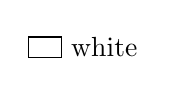
\begin{tikzpicture}
            \colorect{black}{0,1.5}   \colorect{blue}{0,1}   \colorect{brown}{0,.5} \colorect{cyan}{0,0}
            \colorect{darkgray}{2,1.5}\colorect{gray}{2,1}   \colorect{green}{2,.5} \colorect{lightgray}{2,0}
            \colorect{lime}{4,1.5}    \colorect{magenta}{4,1}\colorect{olive}{4,.5} \colorect{orange}{4,0}
            \colorect{pink}{6,1.5}    \colorect{purple}{6,1} \colorect{red}{6,.5}   \colorect{teal}{6,0}
            \colorect{violet}{8,1.5}  \colorect{yellow}{8,.5} \filldraw[draw=black,fill=white](8,1)node[above=4pt,right=1pc,black]{white}rectangle+(1pc,0.618pc);
        \end{tikzpicture}
    \subsubsection{green!60!white}
        \newcommand\colorecti[3]{\fill[#1](#3)node[above=4pt,right=1pc,black]{#2}rectangle+(1pc,0.618pc);}
        \newcommand\colorsix[3]{\colorecti{#1!100!#2}{#1}{#3,2.5}\colorect{#1!80!#2}{#3,2}\colorect{#1!60!#2}{#3,1.5}%
          \colorect{#1!40!#2}{#3,1}\colorect{#1!20!#2}{#3,.5}\colorecti{#1!0!#2}{#2}{#3,0}}%
        \begin{tikzpicture}
            \colorsix{green}{white}{0}
            \colorsix{green}{gray}{4}
            \colorsix{green}{black}{8}
        \end{tikzpicture}\sky\sky
        \begin{tikzpicture}
            \colorsix{green}{red}{0}
            \colorsix{green}{blue}{4}
            \colorsix{green}{yellow}{8}
        \end{tikzpicture}
        \subsubsection{多色混合}
            \begin{tikzpicture}
                \colorect{red}{0,3}  \colorecti{-red!100}{-red}{6,3}
                \colorect{red!75}{0,2.5}  \colorect{-red!75}{6,2.5}
                \colorect{red!75!green}{0,2}  \colorect{-red!75!green}{6,2}
                \colorect{red!75!green!50}{0,1.5}  \colorect{-red!75!green!50}{6,1.5}
                \colorect{red!75!green!50!blue}{0,1}  \colorect{-red!75!green!50!blue}{6,1}
                \colorect{red!75!green!50!blue!25}{0,.5}  \colorect{-red!75!green!50!blue!25}{6,.5}
                \colorect{red!75!green!50!blue!25!gray}{0,0}  \colorect{-red!75!green!50!blue!25!gray}{6,0}
            \end{tikzpicture}
\end{document} 
